%%%%%%%%%%%%%%%%%%%%%%%%%%%%%%%%%%%%%%%%%
% University Assignment Title Page 
% LaTeX Template
% Version 1.0 (27/12/12)
%
% This template has been downloaded from:
% http://www.LaTeXTemplates.com
%
% Original author:
% WikiBooks (http://en.wikibooks.org/wiki/LaTeX/Title_Creation)
%
% License:
% CC BY-NC-SA 3.0 (http://creativecommons.org/licenses/by-nc-sa/3.0/)
% 
% Instructions for using this template:
% This title page is capable of being compiled as is. This is not useful for 
% including it in another document. To do this, you have two options: 
%
% 1) Copy/paste everything between \begin{document} and \end{document} 
% starting at \begin{titlepage} and paste this into another LaTeX file where you 
% want your title page.
% OR
% 2) Remove everything outside the \begin{titlepage} and \end{titlepage} and 
% move this file to the same directory as the LaTeX file you wish to add it to. 
% Then add \documentclass[12pt]{article}
\usepackage[english]{babel}
\usepackage{amsmath}
\usepackage{graphicx}
\usepackage{textcomp}
\usepackage{parskip}
\usepackage[colorinlistoftodos]{todonotes}
\usepackage{csquotes}
\usepackage{float}
\usepackage[backend=biber,style=ieee]{biblatex}
\addbibresource{bibliography.bib}

\begin{document}

\begin{titlepage}

\newcommand{\HRule}{\rule{\linewidth}{0.5mm}}
\center 

\textsc{\LARGE Iowa State University }\\[1.5cm] 
\textsc{\Large Center for Statistics and Applications in Forensic
Evidence
}\\[0.5cm] 

\HRule \\[0.4cm]
{ \huge \bfseries Shoe Print Data Collection: Additional Methods }\\[0.4cm] 
\HRule \\[1.5cm]



\begin{center}
\centering
 
\includegraphics[scale=.4]{csafe-logo}\\[1cm]
\end{center}







\end{titlepage}

\section{Introduction}

 When developing the methodology for the longitudinal shoe study conducted by the Center for Statistics and Applications in Forensic Evidence (CSAFE), collection procedures were designed to obtain the most ideal shoe-sole impression possible. While these images will be useful to the researcher and practitioner communities, they do not provide realistic examples of prints that would be collected from a crime scene/suspected crime scene. For this reason, CSAFE researchers have compiled this manual which contains procedures for further data collection and offers new, or edited, procedures that better represent the practices of current forensic examiners and crime scene teams. If at any time there is a question on any of these procedures, please make a note using a post-it note and e-mail the principal investigator, the project manager, the faculty in charge of the study, or the author of the specific procedure. 

\end{document} to your LaTeX file where you want your
% title page.
%
%%%%%%%%%%%%%%%%%%%%%%%%%%%%%%%%%%%%%%%%%
%\title{Title page with logo}
%----------------------------------------------------------------------------------------
%	PACKAGES AND OTHER DOCUMENT CONFIGURATIONS
%----------------------------------------------------------------------------------------

\documentclass[12pt]{article}
\usepackage[english]{babel}
\usepackage[utf8x]{inputenc}
\usepackage{amsmath}
\usepackage{graphicx}
\usepackage[colorinlistoftodos]{todonotes}

\begin{document}

\begin{titlepage}

\newcommand{\HRule}{\rule{\linewidth}{0.5mm}} % Defines a new command for the horizontal lines, change thickness here

\center % Center everything on the page
 
%----------------------------------------------------------------------------------------
%	HEADING SECTIONS
%----------------------------------------------------------------------------------------

\textsc{\LARGE Iowa State University}\\[1.5cm] % Iowa State University 
\textsc{\Large Center for Statistics and Applications in Forensic Evidence}\\[0.5cm] % CSAFE
\textsc{\large CSAFE }\\[0.5cm] % Center for Statistics and Applications in Forensic Evidence 

%----------------------------------------------------------------------------------------
%	2D Shoe Scanner Procedure
%----------------------------------------------------------------------------------------

\HRule \\[0.4cm]
{ \huge \bfseries 2D Shoe Scanner: Procedure }\\[0.4cm] % Title of your document
\HRule \\[1.5cm]
 
%----------------------------------------------------------------------------------------
%	AUTHOR SECTION
%----------------------------------------------------------------------------------------

\begin{minipage}{0.4\textwidth}
\begin{flushleft} \large
\emph{Author:}\\
James \textsc{E. Kruse} % James E. Kruse
\end{flushleft}
\end{minipage}
~
\begin{minipage}{0.4\textwidth}
\begin{flushright} \large
\emph{Supervisor:} \\
Dr. Guillermo \textsc{Basulto-Elias} % Supervisor's Name
\end{flushright}
\end{minipage}\\[2cm]

% If you don't want a supervisor, uncomment the two lines below and remove the section above
%\Large \emph{Author:}\\
%John \textsc{Smith}\\[3cm] % Your name
%----------------------------------------------------------------------------------------
%	LOGO SECTION
%----------------------------------------------------------------------------------------

\includegraphics[scale=.5]{Logo}\\[1cm]

\begin{center}
\begin{tabular}{ c   |   c } 
 
\end{tabular}
\end{center}
%----------------------------------------------------------------------------------------
%	DATE SECTION
%----------------------------------------------------------------------------------------

{\large \today}\\[2cm] % Date, change the \today to a set date if you want to be precise


 
%----------------------------------------------------------------------------------------

\vfill % Fill the rest of the page with whitespace

\end{titlepage}




\section{Introduction}

The following is the recommended procedure for operating the 2D forensic shoe sole scanner (Figure 1). 

\begin{figure}[!htp]
\centering
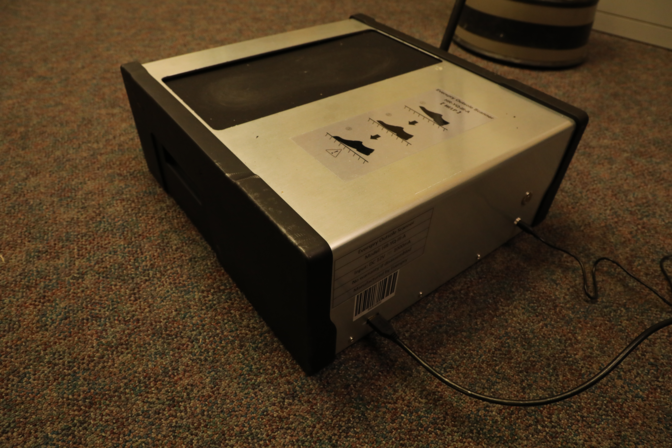
\includegraphics[scale=0.3]{2D_Scanner}
\caption{Everspry Shoe Scanner}
\label{Image 1}
\end{figure}

\subsection{Procedure}

1.	Plug the USB cable, from the 2D scanner, into the computer and its opposite end into the scanner itself.

2.	Position the scanner so that a technician could easily step straight up onto the platform and then step straight off. A nearby wall or person standing next to the scanner can be used for balance. 

3.	Turn on the scanner by pressing the circular button on the right side of the machine. On the desktop, under all programs, search and open EverspryOS.

4.	Before the technician steps up onto the platform, make sure that the acquisition screen is blank and free of previous prints (Figure 2). 

\begin{figure}[!htp]
\centering
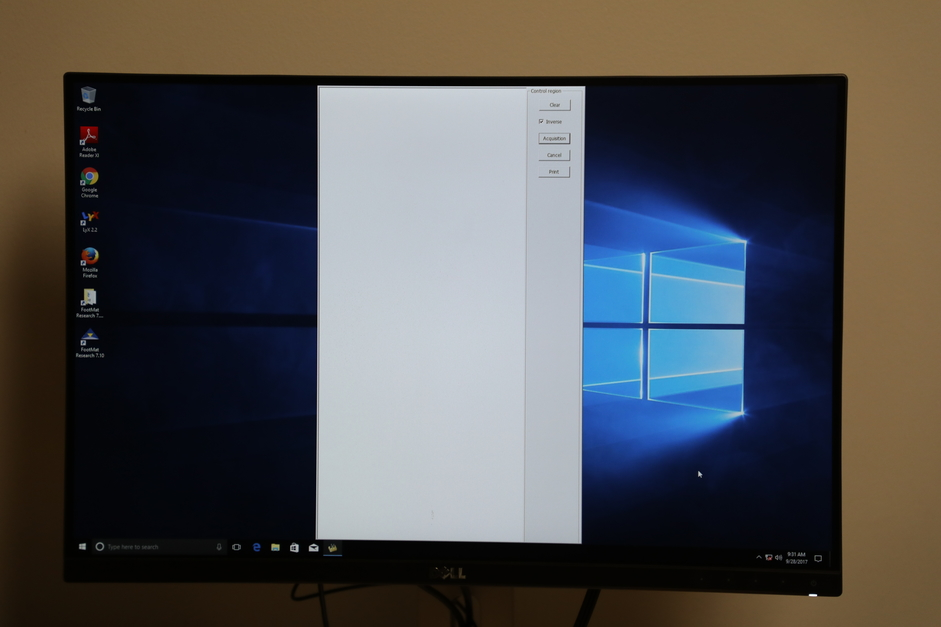
\includegraphics[scale=0.3]{2D_Screen}
\caption{Everspry acquisition screen before a scan is taken}
\label{Image 2}
\end{figure}

\newpage

5. The technician will then put on a pair of disposable socks and the shoe to be scanned.  

6.	When stepping up onto the scanner, the they should place their heel on the scanner with their toe pointing towards the ceiling (Figure 3).  They will then roll their foot into a flat standing position and step up so that all of their weight is on the scanner (Figure 4). 

\begin{figure}[!htp]
\centering
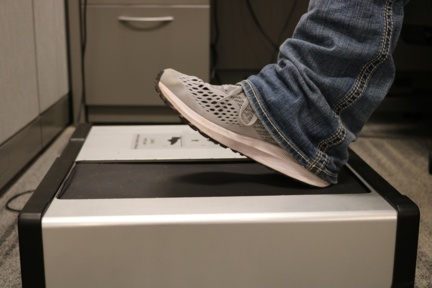
\includegraphics[scale=0.5]{2D_Step_on}
\caption{Technician Stepping up onto the scanner}
\label{Image 3}
\end{figure}


\begin{figure}[!htp]
\centering
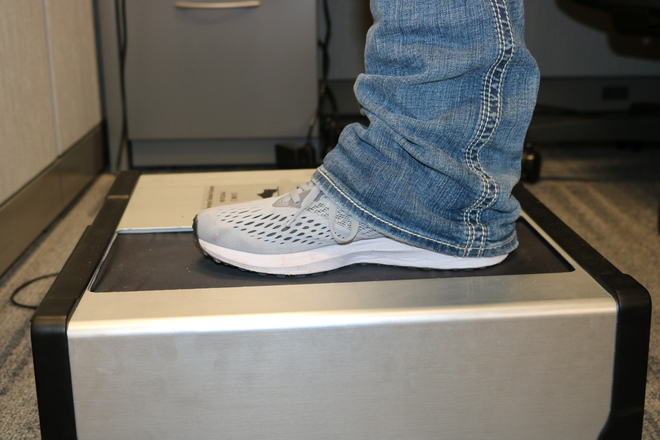
\includegraphics[scale=0.3]{Stand_on_2D}
\caption{Technician placing their foot flat on the scanner}
\label{Image 4}
\end{figure}

\newpage

7.	Shift weight in the shoe in order to capture all detail possible. Make sure that the shoe is not double printed. 

8.	Carefully, have the technician step off of the scanner. Peel the foot forward until only the tip of the toe is making contact with the platform. At this point, lift the foot straight up, off of the scanner (Figure 5). 

\begin{figure}[!htp]
\centering
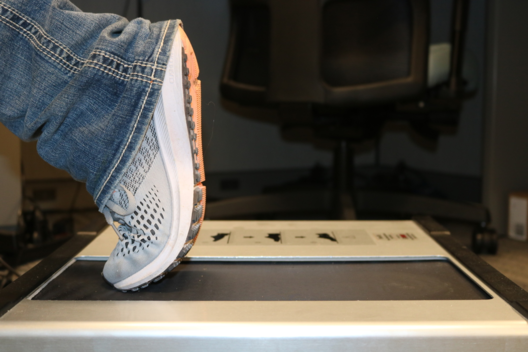
\includegraphics[scale=0.3]{2D_Step_off}
\caption{Technician stepping off of the scanner}
\label{Image 5}
\end{figure}


9.	Review the print on the acquisition screen and if it is clear, complete, and free of smudges/overlap, press acquisition. If the image is not suitable, press clear and repeat the scanning procedure (Figure 6).  

\begin{figure}[!htp]
\centering
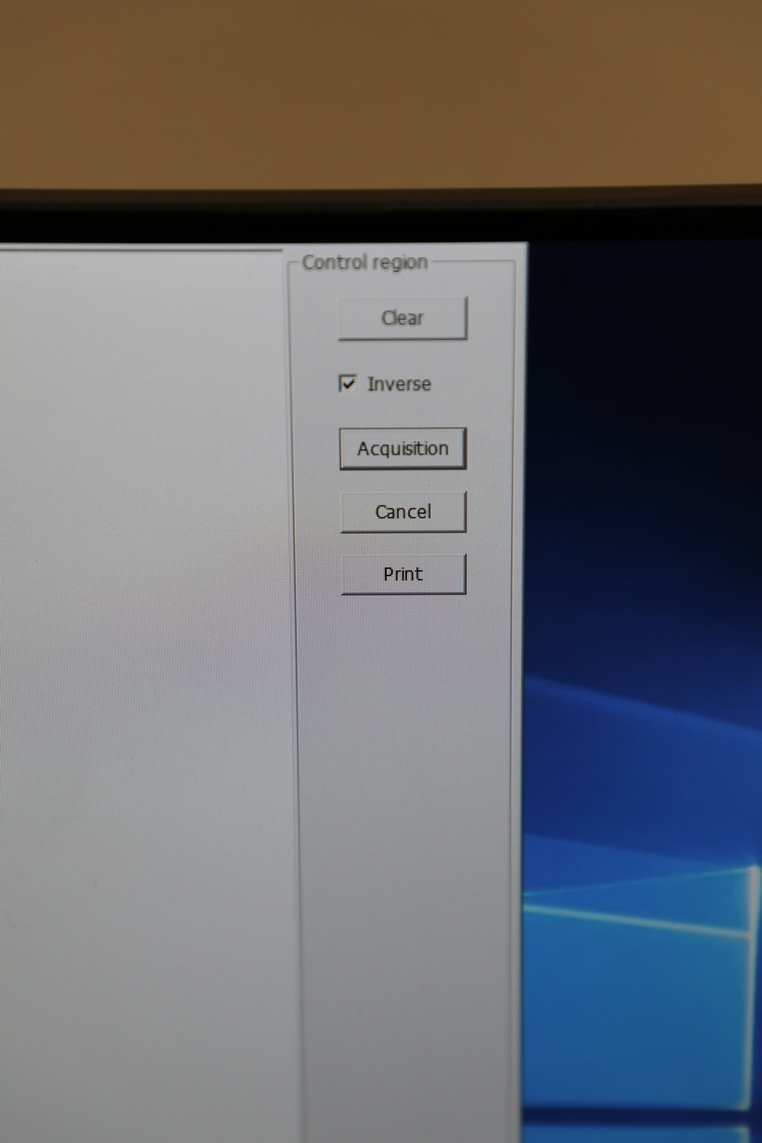
\includegraphics[scale=0.2]{2D_Screen_2}
\caption{Close up view of the acquisition screen}
\label{Image 6}
\end{figure}

\newpage

10. Save the image (Figure 7) as a tiff file. Use the tool created by IT to generate a name for the image using the key on the backside of the cover of this manual. Repeat this procedure for the "detailed image" twice for each shoe. 

\begin{figure}[!htp]
\centering
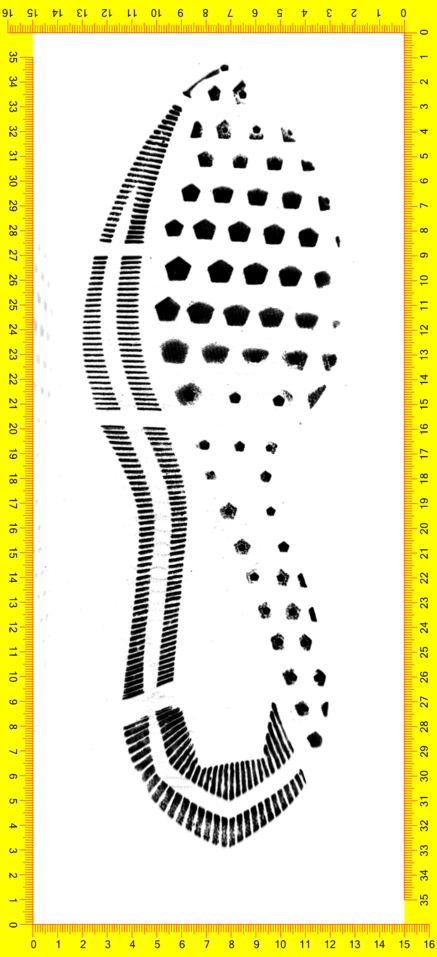
\includegraphics[scale=.9]{2D_1}
\caption{Sample of the first step 2D scan}
\label{Image 7}
\end{figure}

\newpage

11. For the second image type, have the technician walk across the scanner as if walking down the street. They will step up onto the scanner and then right back off. No attempt should be made to create a perfect print, as this image is meant to capture a realistic step (Figure 8). 

\begin{figure}[!htp]
\centering
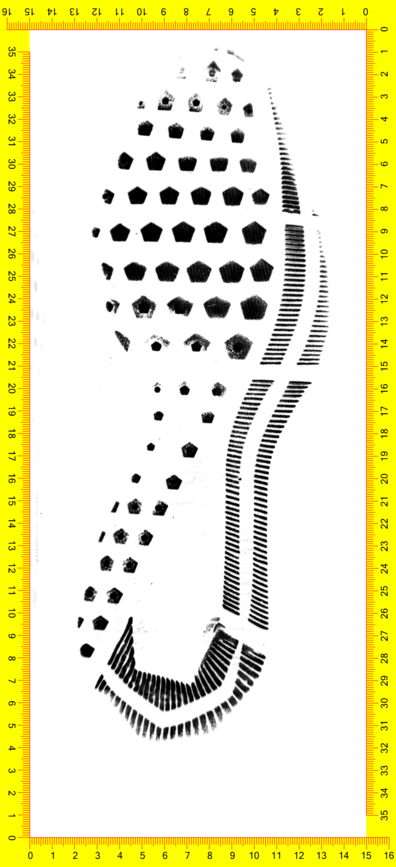
\includegraphics[scale=.9]{2D_2}
\caption{Sample of second step 2D scan}
\label{Image 8}
\end{figure}

\newpage

12. Save the image as a tiff file. Use the tool created by IT to generate a name for the image using the key on the backside of the cover of this manual. Repeat this procedure for the "walking image" twice for each shoe. 

10. When one pair of shoe is finished, there will be 8 Tiff images. 

Note: Please do not use any type of liquid on the scanner Pad to clean it. Please contact James Kruse from CSAFE or Larry from CSSM. No water, sprays, wipes, etc. can be used. 

\end{document}

